\documentclass{article}
\usepackage[letterpaper, top=1in, bottom=1in, left=1in, right=1in]{geometry}
\usepackage[utf8]{inputenc}


\usepackage[english]{babel}
\usepackage{tikz-cd, pgfplots, lipsum, bm, dcolumn}
\usepackage{amsmath, amssymb, amsthm, mathrsfs, mathtools, centernot, hyperref, fancyhdr, lastpage}
\usepackage{graphicx} 
\usepackage{caption, subcaption}
\usepackage{enumitem}
\usepackage{fancyvrb,newverbs,xcolor}
\usepackage{tikz}
\usetikzlibrary{matrix}
\definecolor{cverbbg}{gray}{0.93}

\newenvironment{cverbatim}
 {\SaveVerbatim{cverb}}
 {\endSaveVerbatim
  \flushleft\fboxrule=0pt\fboxsep=.5em
  \colorbox{cverbbg}{%
    \makebox[\dimexpr\linewidth-2\fboxsep][l]{\BUseVerbatim{cverb}}%
  }
  \endflushleft
}

\renewcommand{\thispagestyle}[1]{}


\theoremstyle{definition}
\newtheorem{theorem}{Theorem}[section]
\newtheorem{proposition}[theorem]{Proposition}
\newtheorem{lemma}[theorem]{Lemma}
\newtheorem{example}{Example}[section]
\newtheorem{exercise}{Exercise}[section]
\newtheorem{corollary}{Corollary}[theorem]
\theoremstyle{remark}
\newtheorem*{remark}{Remark}
\theoremstyle{definition}
\newtheorem{definition}{Definition}[section]
\renewcommand{\qed}{\hfill$\blacksquare$}
\renewcommand{\footrulewidth}{0.4pt}% default is 0pt

\newenvironment{solution}{\noindent \textit{Solution.}}{}

\renewcommand{\thispagestyle}[1]{}


\begin{document}
\pagestyle{fancy}

\lhead{Computer Vision}
\chead{Muchang Bahng}
\rhead{\date{Summer 2023}}
\cfoot{\thepage / \pageref{LastPage}}

\title{Computer Vision}
\author{Muchang Bahng}

\maketitle

\tableofcontents

\pagebreak


\section{Cameras and Transformations}

\subsection{Lie Groups and Lie Algebras}

\subsection{Camera Parameterizations}

\subsection{Sampling and Quantization}

\subsection{Image Compression}


\section{Image Processing}

\subsection{Basic Functionality}

A pixel can be really represented by a number. More specifically, a grayscale pixel is a number between $0$ (black) and $255$ (white), and a color pixel is in the RGB format, represented by a $3$-tuple. Therefore, a grayscale image is really represented by a $H \times W$ matrix, and a RBG image by a $3 \times H \times W$ tensor. We can see this when opening up an image in OpenCV with the following code: 
\begin{cverbatim}
import cv2 

PATH = "park.jpg"

img = cv2.imread(PATH)
gray = cv2.cvtColor(img, cv2.COLOR_BGR2GRAY) 

cv2.imshow("Park", img)     # Show RGB image
cv2.imshow('Gray', gray)    # Show gray image
cv2.waitKey(0)              # Wait time until image closes
\end{cverbatim}
The results are shown in Figure \ref{fig:Park_Images}. 

\begin{figure}[hbt!]

    \centering
    \begin{subfigure}[b]{0.45\textwidth}
    \centering
        \includegraphics[width=\textwidth]{Images/OpenCV/Gray_Full.png}
        \caption{Gray picture of park}
        \label{fig:1d}
    \end{subfigure}
    \begin{subfigure}[b]{0.45\textwidth}
    \centering
        \includegraphics[width=\textwidth]{Images/OpenCV/Gray_Cropped.png}
        \caption{Gray channel}
        \label{fig:2d}
    \end{subfigure}

    \centering
    \begin{subfigure}[b]{0.45\textwidth}
    \centering
        \includegraphics[width=\textwidth]{Images/OpenCV/Park_Full.png}
        \caption{Colored picture of park}
        \label{fig:3d}
    \end{subfigure}
    \begin{subfigure}[b]{0.45\textwidth}
    \centering
        \includegraphics[width=\textwidth]{Images/OpenCV/Park_Cropped.png}
        \caption{RGB channels}
        \label{fig:4d}
    \end{subfigure}
    \label{fig:Park_Images}
    \caption{Different color channel representations of an image. }
\end{figure}

The $\texttt{img}$ object called by $\texttt{cv2.imread()}$ actually outputs a numpy array directly. This makes it easy for us to access the resolution of the image and to crop it by slicing across the dimensions. We can also rescale it accordingly using $\texttt{cv.resize()}$. 
\begin{cverbatim}
print(img.shape)        <class 'numpy.ndarray'> (427, 640, 3)
print(gray.shape)       <class 'numpy.ndarray'> (427, 640)

# Crop it 
img_cropped = img[100:200, 100:200, :]

# Resize the image 
width, height = int(frame.shape[1] * 0.6), int(frame.shape[0] * 0.6) 
dimensions = (width, height) 
img_resized = cv2.resize(img, dimensions, interpolation=cv2.INTER_AREA) 
\end{cverbatim}

\subsubsection{Color Histograms}

You can also find the distribution of the color channels in an image with a histogram. A code snippet is shown below, along with the corresponding generated plots in Figure \ref{fig:cats_histogram}. 
\begin{cverbatim}
img = cv2.imread("Cats.jpg)
cv2.imshow("Cats", img) 

# Color histogram 
colors = ('b', 'g', 'r') 
for i, col in enumerate(colors): 
    hist = cv2.calcHist([img], [i], None, [256], [0, 256]) 
    plt.plot(hist, color=col) 
    plt.xlim([0, 256]) 
    
plt.show() 
cv2.waitKey(0) 
\end{cverbatim}

\begin{figure}[hbt!]
    \centering
    \begin{subfigure}[b]{0.45\textwidth}
    \centering
        \includegraphics[width=\textwidth]{Images/OpenCV/Cats.png}
        \caption{Gray picture of park}
        \label{fig:5d}
    \end{subfigure}
    \begin{subfigure}[b]{0.45\textwidth}
    \centering
        \includegraphics[width=\textwidth]{Images/OpenCV/Cats_color_hist.png}
        \caption{Gray channel}
        \label{fig:6d}
    \end{subfigure}
    \label{fig:cats_histogram}
    \caption{RBG Channel Histograms for Cats.png image. }
\end{figure}


\subsection{Drawing and Transformations}

\subsubsection{Masking}

\subsection{Kernels}

Now a convolution is described by a \textbf{kernel}, also called a \textbf{filter}, which is simply a $K \times K$ matrix. It does not have to be square but is conventionally so. It goes through a grayscale image at every point and compute the dot product of the kernel with the overlapping portion of the image, creating a new pixel. This can be shown in Figure \ref{fig:convolution1}. 

\begin{figure}
\centering
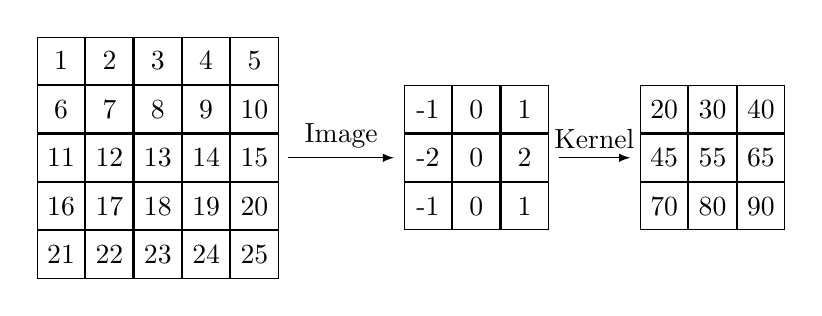
\begin{tikzpicture}[>=latex]

% Image
\matrix[matrix of nodes, nodes={draw, minimum size=0.6cm, anchor=center}] (image) {
    1 & 2 & 3 & 4 & 5 \\
    6 & 7 & 8 & 9 & 10 \\
    11 & 12 & 13 & 14 & 15 \\
    16 & 17 & 18 & 19 & 20 \\
    21 & 22 & 23 & 24 & 25 \\
};

% Kernel
\matrix[matrix of nodes, nodes={draw, minimum size=0.6cm, anchor=center}, right=3cm] (kernel) {
    -1 & 0 & 1 \\
    -2 & 0 & 2 \\
    -1 & 0 & 1 \\
};

% Convolution result
\matrix[matrix of nodes, nodes={draw, minimum size=0.6cm, anchor=center}, right=6cm] (result) {
    20 & 30 & 40 \\
    45 & 55 & 65 \\
    70 & 80 & 90 \\
};

% Arrows
\draw[->] (image) -- node[midway, above] {Image} (kernel);
\draw[->] (kernel) -- node[midway, above] {Kernel} (result);

\end{tikzpicture}
\caption{Convolution using a kernel on an image.}
\label{fig:convolution1}
\end{figure}

Now if this was a color image, then the $K \times K$ kernel $\mathcal{K}$ would dot over all 3 layers, without changing over all 3 layers. This is equivalent to applying the kernel over all 3 channels separately, and then combining them together into one. Another thing to note is that the output image of a kernel would be slightly smaller than the input image, since the kernel cannot go over the edge. However, there are padding schemes to preserve the original dimensions. To construct our custom kernel, we can simply create a custom matrix: 
\begin{cverbatim}
img = cv2.imread("cats.jpg")

# create custom 5x5 kernel
kernel = (1/25) * np.ones((5, 5), dtype=np.float32)

# apply to image
dst = cv2.filter2D(img, -1, kernel)
cv2.imshow("Park", dst)
cv2.waitKey(0)
\end{cverbatim}
Note that the kernel matrix may have the property that all of its entries sum to $1$, meaning that on average, the expected value of the brightness of each pixel will be $0$, and the values will be left unchanged on average. However, this is not a requirement. 

\begin{example}[Mean Blur, Gaussian Blur]
The mean and Gaussian blur is defined with kernels that are distributed uniformly and normally across the entire matrix. You can see how this would blur an image since for every pixel, we take the weighted average over all of its surrounding pixels. 
\[\text{mean} = \frac{1}{25} \begin{bmatrix} 1 & 1 & 1 & 1 & 1 \\ 1 & 1 & 1 & 1 & 1 \\ 1 & 1 & 1 & 1 & 1 \\ 1 & 1 & 1 & 1 & 1 \\ 1 & 1 & 1 & 1 & 1 \end{bmatrix}, \;\;\;\;\; \text{Gaussian} = \frac{1}{273} \begin{bmatrix} 1 & 4 & 7 & 4 & 1 \\ 4 & 16 & 26 & 16 & 4 \\ 7 & 26 & 41 & 26 & 7 \\ 4 & 16 & 26 & 16 & 4 \\ 1 & 4 & 7 & 4 & 1 \end{bmatrix}\]
On a large scale, there really aren't any discernable differences, as seen in Figure \ref{fig:blur}, but the Guassian blur is known to be a more realistic representation of how humans receive blur. 
\begin{figure}[hbt!]
    \centering
    \begin{subfigure}[b]{0.32\textwidth}
    \centering
        \includegraphics[width=\textwidth]{Images/OpenCV/Park_Full.png}
        \caption{Original image. }
        \label{fig:d}
    \end{subfigure}
    \begin{subfigure}[b]{0.32\textwidth}
    \centering
        \includegraphics[width=\textwidth]{Images/OpenCV/Mean_Blur.png}
        \caption{$5 \times 5$ mean blur applied. }
        \label{fig:d}
    \end{subfigure}
    \begin{subfigure}[b]{0.32\textwidth}
    \centering
        \includegraphics[width=\textwidth]{Images/OpenCV/Gaussian_Blur.png}
        \caption{$5 \times 5$ Gaussian blur applied. }
        \label{fig:d}
    \end{subfigure}

    
    \caption{Comparison of blurring kernels on image. }
    \label{fig:blur}
\end{figure}
\end{example}

\begin{example}[Sharpening]
A sharpening of an image would be the opposite of a blur, meaning that we emphasize the center pixel and reduce the surrounding pixels. 
\[\text{Sharpen} = \begin{bmatrix} 0 & -1 & 0 \\ -1 & 5 & -1 \\ 0 & -1 & 0 \end{bmatrix}\]
\begin{figure}[hbt!]
    \centering
    \begin{subfigure}[b]{0.45\textwidth}
    \centering
        \includegraphics[width=\textwidth]{Images/OpenCV/Park_Full.png}
        \caption{Original image. }
        \label{fig:d}
    \end{subfigure}
    \begin{subfigure}[b]{0.45\textwidth}
    \centering
        \includegraphics[width=\textwidth]{Images/OpenCV/Sharpen.png}
        \caption{$3 \times 3$ sharpening applied. }
        \label{fig:d}
    \end{subfigure}

    \label{fig:cats_histogram}
    \caption{Sharpening kernels applied to image. }
\end{figure}
\end{example}

\begin{example}[Edge Detection]
The edge detecting kernel looks like the following, which differs for horizontal and vertical edge detection. Note that the sum of all of its values equal $0$, which means that for areas that have a relatively constant value of pixels, all the surrounding ones will ``cancel" out and the kernel will output a value of $0$, corresponding to black. This is why we see mostly black in the photo. 
\[\text{Horizontal} = \begin{bmatrix} -1 & 0 & 1 \\ -2 & 0 & 2 \\ -1 & 0 & 1 \end{bmatrix}, \;\;\;\;\;\; \text{Vertical} = \begin{bmatrix} -1 & -2 & -1 \\ 0 & 0 & 0 \\ 1 & 2 & 1 \end{bmatrix}\]
\begin{figure}[hbt!]
    \centering
    \begin{subfigure}[b]{0.45\textwidth}
    \centering
        \includegraphics[width=\textwidth]{Images/OpenCV/Horizontal.png}
        \caption{$3 \times 3$ horizontal edge detecting kernel applied. }
        \label{fig:d}
    \end{subfigure}
    \begin{subfigure}[b]{0.45\textwidth}
    \centering
        \includegraphics[width=\textwidth]{Images/OpenCV/Vertical.png}
        \caption{$3 \times 3$ vertical edge detecting kernel applied. }
        \label{fig:d}
    \end{subfigure}

    \label{fig:cats_histogram}
    \caption{Edge detecting kernels applied to image. }
\end{figure}
\end{example}

\section{Region Based Object Detection}

So far, we can use CNNs to either classify or regress an input image. However, the task of \textbf{object detection} requires us to draw bounding boxes around an arbitrary number of objects within an image \textit{and} correctly label each one. This seems like quite an enormous task, but we can build it up step by step. 

\subsection{RCNN}



\subsection{Fast RCNN}

\subsection{Faster RCNN}

\subsection{Mask RCNN}

\section{YOLO}

\section{Simple Online Realtime Tracking} 

\subsection{SORT}

\subsection{DeepSORT}

\subsection{StrongSORT}

\section{ByteTrack}




\end{document}
